\begin{definition}[Point Mutation]
    The \textit{point mutation} operator in GP works by picking a random node in a program tree and replacing it 
    with another node that has the same number of child nodes (arity). This swap creates a variation of the original 
    program while keeping the overall tree structure intact.

    The operation can be mathematically represented as:

    \begin{equation}
        M_{point}(P: \mathbb{P},\, \mu_\textbf{i}: [0,\, 1],\, \mu_\textbf{c}: [0,\, 1],\, \mu_\textbf{g}: [0,\, 1])
            \to \mathbb{P}
    \end{equation}

    Explaining the parameters:

    \begin{itemize}
        \item \(P\): The population of program trees.
        \item \(\mu_\textbf{i}\): The chance of mutating an individual tree.
        \item \(\mu_\textbf{c}\): The chance of mutating a chromosome within a tree.
        \item \(\mu_\textbf{g}\): The probability of selecting a particular gene for mutation.
    \end{itemize}
\end{definition}

The implementation of the Point Mutation operator in \textit{Keen} follows a four-step process:

\begin{code}{
    Example of Point Mutation in \textit{Keen}
}{label=lst:keen:gp:op:mutation:point}{kotlin}
    val original = random node in program tree
    val replacements = nodes with same arity as original
    val replacement = random node in replacements
    val mutated = program tree with original replaced by replacement
\end{code}

A key feature of Point Mutation in \textit{Keen} is its ability to maintain the overall structure of program trees 
while introducing genetic changes.

\begin{remark}
    The focus on matching arity during node replacement is important. This method ensures the mutated tree retains 
    the structure of the original tree, reducing the chances of runtime errors or unclear meanings that could hinder 
    the evolutionary process.
\end{remark}

A visual example of how the Point Mutation operator works is shown in \vref{fig:keen:gp:op:mutation:point}.

\begin{figure}[ht!]
    \centering
    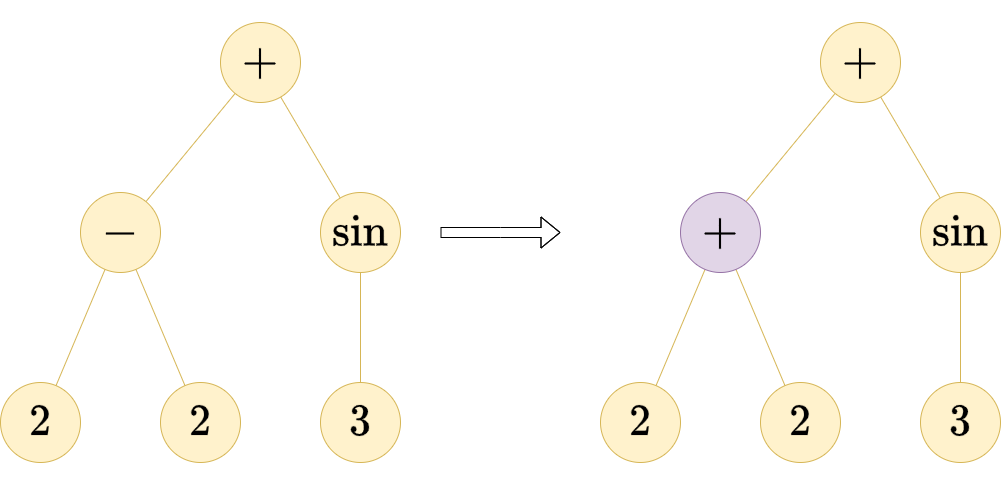
\includegraphics[width=0.5\textwidth]{img/keen/Point mutation.png}
    \caption{
        A graphical elucidation of the Point Mutation operator's effect on a program tree. A random node is selected 
        and substituted with another of identical arity, resulting in a structurally-consistent variant of the 
        original tree.
    }
    \label{fig:keen:gp:op:mutation:point}
\end{figure}
